\chapter{Stand des Wissens und der Technik}
\section{Funktionsweise eines Prozessors}

Ein Prozessor ist eine universelle Rechnermaschine, die sich durch eine definierte Reihe von Anweisungen programmieren lässt. Zu den arithmetischen Anweisungen gehören der Zugriff auf Speicheradressen und Sprünge innerhalb der Abfolge der Anweisungen.
Bereits der britische Mathematiker Alan Turing konnte aufzeigen, dass ein universelles Berechnungsmodell möglich ist, wenn ein Rechner neben Speicherzugriff auch Sprünge besitzt\cite{Hoffmann2014l}. Auf diesen besonderen Eigenschaften bauen die heutigen Prozessoren auf. Ein Programm, das den Prozessor ansteuert, besteht aus einer endlichen Anzahl von geordneten Anweisungen. Der Prozessor befolgt, streng nach dem Ablauf, Anweisung für Anweisung, die auch Sprünge zu anderen Stellen innerhalb des Programms besitzen.
\par
Die Prozessoren, auch Zentraleinheiten oder CPUs genannt, besitzen im Inneren drei Einheiten, die über einen Datenbus verbunden sind. Dies ist in der \autoref{fig:CPU} ersichtlich. Dabei kann der Datenbus je nach Grösse oder Leistung des CPUs variieren. Die meist verbreiteten CPUs, die in den heutigen PC verbaut sind, haben einen 64bit-Datenbus. In dieser Arbeit wird aber mit kleineren CPUs gearbeitet, die einen 32bit-Datenbus besitzen. Die Control Unit\cite{patterson2013computer} ist dafür verantwortlich, dass das Programm immer an der richtigen Stelle ausgeführt wird. Sie nimmt Anweisungen an, dekodiert diese und übergibt sie der ALU. Die Übergabe der Daten an die ALU und die Register erfolgt durch die Weichenstellung des Datenbusses. Die Arithmetic and Logical Unit (ALU) ermöglicht es, Rechenoperationen sowie logische Operationen an den Daten auszuführen. Die Register haben die Grösse des Datenbusses und dienen dazu, die Daten von und zur ALU zu bewegen. Eine CPU besitzt mehrere Register, die je nach CPU-Architektur variieren. Die Register lassen sich in zwei Kategorien, Universal- und Hilfsregister, unterteilen. In den Universalregistern lassen sich die zu bearbeitenden Daten speichern. Die Hilfsregister haben eine besondere Rolle zugeordnet erhalten. Beispielsweise zählt das Statusregister zu den Hilfsregistern. Dieses spezielle Hilfsregister gibt Aufschluss über das Resultat der vorherigen Operation. So lässt sich über dieses Hilfsregisters herauslesen, ob eine Operation von zwei Zahlen den möglichen Speicherplatz des Registers übersteigt und es zu einem sogenannten "overflow" kommt.
Da die Anzahl meist sehr klein ist, müssen die Daten immer wieder von den Registern in den RAM und wieder zurückgeladen werden.
\par
Prozessoren sind als elektronische Schaltkreise realisiert. Die Schaltkreise werden durch die Halbleitertechnologie hergestellt. Die Millionen von witzigen Transistoren, die ein Prozessor beinhaltet, werden zu logischen Bausteinen verdrahtet.
\par
In dieser Arbeit ist die Funktionsweise der ALU relevant. Wir wissen, dass die ALU eine Reihe von Anweisungen erhält und somit jeden erdenklichen Algorithmus ausführen kann. Im Rahmen dieser Arbeit wird eine Methode entwickelt, um den Energieverbrauch einer einzelnen Anweisung der ALU messen können.



\begin{figure}[t]
\centering
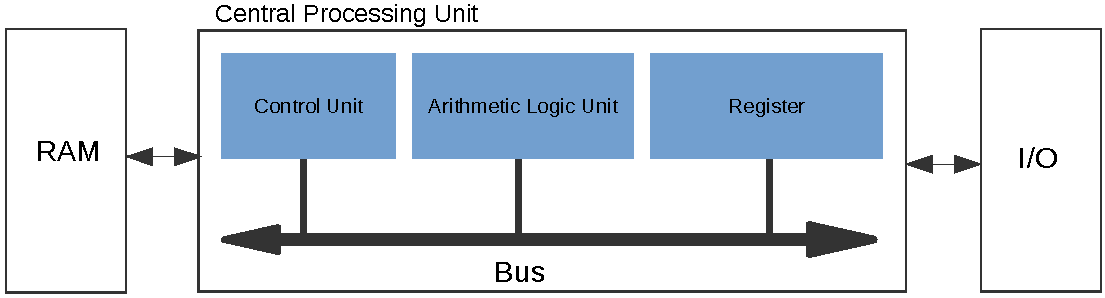
\includegraphics[width=1.0\textwidth]{images/cpu.pdf}
\caption{Central Processing Unit}
\label{fig:CPU}
\end{figure}

\section{Aufbau des Linux Betriebssystem}


\section{Unterschiede CISC und RISC CPUs}



\section{Energy Storage in a Capacitor}


